\documentclass{article}
%\usepackage[spanish,activeacute]{babel}
%\usepackage[english,activeacute]{babel}
%\usepackage[latin1]{inputenc}
\usepackage[utf8]{inputenc}
\usepackage[english]{babel}

\usepackage{amsmath,amsfonts,amssymb,amstext,amsthm,amscd}
\usepackage{hyperref}
\usepackage{latexsym}
\usepackage{graphicx}
%\usepackage{subfigure}
\usepackage{subfig}
%\linespread{1.6}
\usepackage{float}
\usepackage{dcolumn}% Align table columns on decimal point(esto lo saque del ejemplo de revtex4)
\usepackage{bm}% bold math(esto lo saque del ejemplo de revtex4)
\newcounter{itemR}
\usepackage{here} %recordar usar el comando[H] para las gráficas que es el comando here en lugar de [h!]
\usepackage{fancyhdr}
%\usepackage{sidecap}
%\usepackage[spanish,activeacute]{babel}
\usepackage{multirow}
\usepackage{multicol}
\usepackage{array}
\usepackage{enumitem}
%\usepackage{booktabs}% para hacer tablas profesionales con \toprule

% ------------------------------------------------------------------------------------------------------------------------------------------------------

\usepackage{fancyhdr}
\setlength{\headheight}{15.2pt}
\usepackage[paperwidth=8.5in, paperheight=11.0in, top=1.0in, bottom=1.0in, left=1.0in, right=1.0in]{geometry}

\pagestyle{fancyplain}
\fancyhead[LE,RO]{Práctica $\#$9}
\fancyhead[CE,CO]{}
\fancyhead[RE,LO]{P23-FIS1012-12}
\fancyfoot[LE,RO]{\thepage}
\fancyfoot[CE,CO]{Laboratorio de Física, UDLAP}
\fancyfoot[RE,LO]{}

% ------------------------------------------------------------------------------------------------------------------------------------------------------
% ------------------------------------------------------------------------------------------------------------------------------------------------------
% ------------------------------------------------------------------------------------------------------------------------------------------------------

\begin{document}

\fancypagestyle{plain}{
   	\renewcommand{\headrulewidth}{1pt}
   	\renewcommand{\footrulewidth}{1pt}
}

\renewcommand{\footrulewidth}{1pt}
\renewcommand{\tablename}{Tabla}
\renewcommand{\figurename}{Figura}

% ------------------------------------------------------------------------------------------------------------------------------------------------------
% ------------------------------------------------------------------------------------------------------------------------------------------------------
% ------------------------------------------------------------------------------------------------------------------------------------------------------

\title{Circuito RC}
\author{\small{Luis Alberto Gil Bocanegra ID: 177410, Erick Gonzalez Parada ID: 178145}\\
 \small{Gartzen Aldecoa Barroso ID: 178034 .}\\		% ----- Varios autores separarlos por comas:  \small{Nombre(s) de (los) autor(es)\footnote{ID; correo@udlap.mx}, Nombre(s) de (los) autor(es)\footnote{ID; correo@udlap.mx}
	   \small{Depto. de Actuaría, Física y Matemáticas, Universidad de las Américas Puebla, Puebla, M\'exico 72810}}
\date{\small{\today}}

\maketitle

% ------------------------------------------------------------------------------------------------------------------------------------------------------
% ------------------------------------------------------------------------------------------------------------------------------------------------------
% ------------------------------------------------------------------------------------------------------------------------------------------------------

\begin{abstract}
La práctica consistió en entender el funcionamiento de los capacitores y su objetivo principal de ellos que es almacenar carga
, se obtuvieron gráficas con comportamientos correctos.
\\
\\
{\it Keywords:}  voltaje, capacitor 
\\
\\
\end{abstract}

% ------------------------------------------------------------------------------------------------------------------------------------------------------

\begin{multicols}{2}
\section{Desarrollo teórico}\label{Desarrollo Teorico}                              	% -------------------- Introducción
Nuestro objetivo fue observar como el capacitor empieza a perder la carga con forme al tiempo cuando desconectamos el circuito de la corriente.
\cite{Moebs}
Un circuito RC consiste en un resistor y un capacitor conectados en serie o en paralelo. Los capacitores almacenan carga eléctrica y presentan una resistencia al flujo de corriente en corriente alterna pero no en continua.
\begin{equation}
R\left(\frac{dq(t)}{dt}\right) + \frac{q(t)}{C} = V_{fem}
\end{equation}
Donde:
R es la resistencia del resistor en Ohms ($\Omega$)
q(t) es la carga acumulada en el capacitor en función del tiempo en Coulombs (C)
C es la capacidad del capacitor en Faradios (F)
$V_{fem}$ es la fuente de tensión aplicada en Voltios (V)
\section{Desarrollo Experimental}\label{Desarrollo experimental}				% -------------------- Metodología 
\subsection*{Lista de Materiales}
A continuación se presenta una lista de materiales:
\begin{enumerate}
    \item Interface universal UI-500
    \item Sensor de voltaje
    \item Fuente de bajo voltaje 0-24V
    \item Multímetro 
    \item Capacitores 
    \item Resistencias 
    \item Cables banana-Caiman
\end{enumerate}
Se armo el circuito con diferentes capacitores cada vez, en donde alimentamos nuestro circuito realizamos lo que es desconectar
el voltaje para observar como la carga del capacitor empieza a disminuir con cada diferente capacitor y graficamos con un software.
\end{multicols}
\section{Resultados y análisis}\label{Resultados}			% -------------------- Resultados
De todo el muestreo obtuvimos las siguientes gráficas
\begin{figure}[H]
   \centering 
   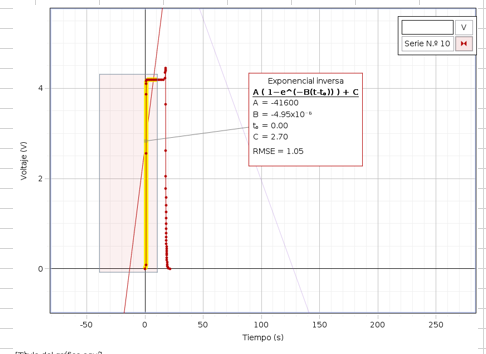
\includegraphics[scale=0.5]{../imgs/r.png}
   \caption{Capacitor 1 C=390k}
   \label{Fig:1}
\end{figure}

\begin{figure}[H]
   \centering 
   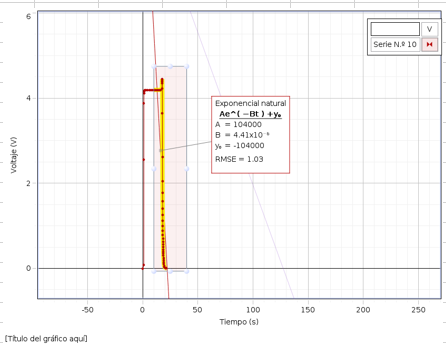
\includegraphics[scale=0.5]{../imgs/r1.png}
   \caption{Capacitor 1 C=390k}
   \label{Fig:2}
\end{figure}

\begin{figure}[H]
   \centering 
   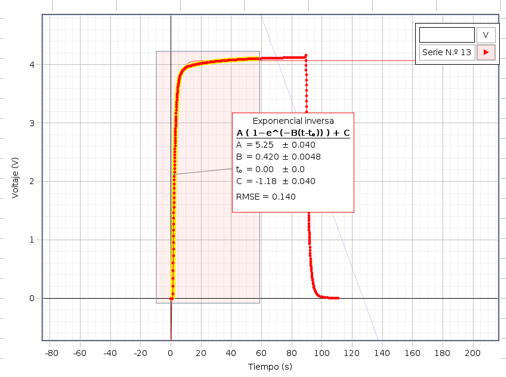
\includegraphics[scale=0.5]{../imgs/r2.png}
   \caption{Capacitor 2 C=2.2mF}
   \label{Fig:3}
\end{figure}

\begin{figure}[H]
   \centering 
   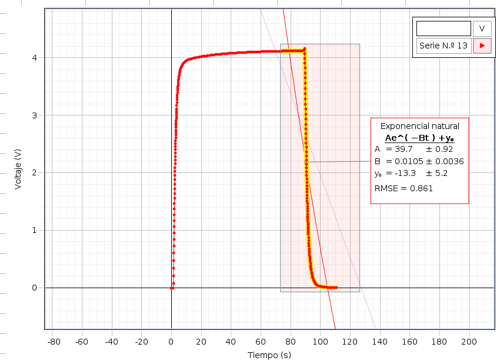
\includegraphics[scale=0.5]{../imgs/r3.png}
   \caption{Capacitor 2 C=2.2mF}
   \label{Fig:4}
\end{figure}

\begin{figure}[H]
   \centering 
   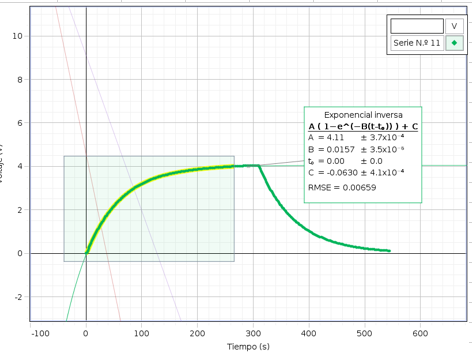
\includegraphics[scale=0.5]{../imgs/r4.png}
   \caption{Capacitor 3 C=100mF}
   \label{Fig:5}
\end{figure}

\begin{figure}[H]
   \centering 
   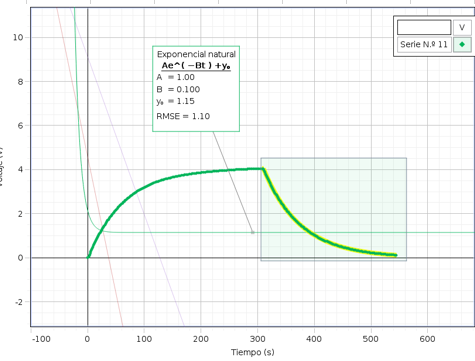
\includegraphics[scale=0.5]{../imgs/r5.png}
   \caption{Capacitor 3 C=100mF}
   \label{Fig:6}
\end{figure}

\begin{figure}[H]
   \centering 
   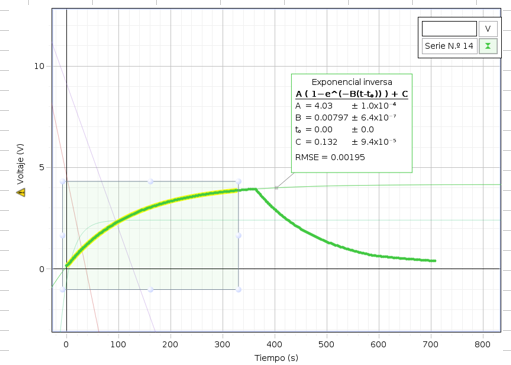
\includegraphics[scale=0.5]{../imgs/r6.png}
   \caption{Capacitor 4 C=220mF}
   \label{Fig:7}
\end{figure}

\begin{figure}[H]
   \centering 
   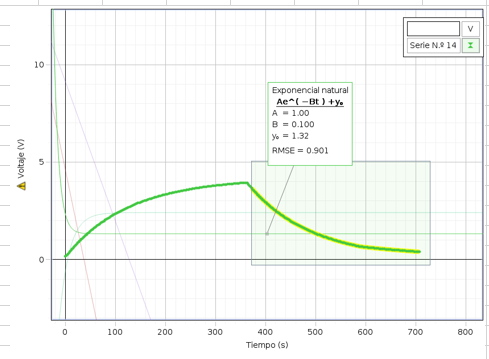
\includegraphics[scale=0.5]{../imgs/r7.png}
   \caption{Capacitor 4 C=220mF}
   \label{Fig:8}
\end{figure}

La razón por la cual ninguno de los valores de B calculados se acercó al resultado obtenido durante la práctica es debido al mal muestreo de los datos. Sin embargo, el comportamiento de la gráfica si es el adecuado.
\section{Conclusiones}\label{Conclusiones}				% -------------------- Conclusiones
El objetivo si se cumplió, como se pudo observar en las gráficas y como ya mencionado el comportamiento de nuestros datos es el correcto, por otro lado,
en resumen, los capacitores son dispositivos que pueden acumular carga eléctrica en sus placas cuando se conectan a una fuente de voltaje, y esta carga se almacena en forma de energía electrostática. Sin embargo, cuando se desconecta la fuente de voltaje, los capacitores eventualmente descargan esa energía a través de un proceso llamado "descarga" a través de una resistencia interna y externa. Por lo tanto, la carga almacenada disminuirá con el tiempo hasta que el capacitor esté completamente descargado. Este proceso es esencial en muchos circuitos electrónicos, como filtros y temporizadores, y es una propiedad fundamental de los capacitores en electrónica.


\begin{thebibliography}{9}						% -------------------- Bibliografía
	\bibitem{Moebs}
 Moebs, W. (2021, 17 noviembre). 10.5 Circuitos RC - Física Universitaria Volumen 2 | OpenStax. https://openstax.org/books/f\%C3\%ADsica-universitaria-volumen-2/pages/10-5-circuitos-rc
	\bibitem{Serway}
	Serway, R. A., $\&$ Jewett, J. W. (2008). Física para ciencias e ingeniería. (7.a
ed., Vol. 1). CENGAGE Learning.

\bibitem{Pérez}
	Newton, I. (1687). Philosophiæ Naturalis Principia Mathematica [Mathematical Principles of Natural Philosophy]. Londini: Jussu Societatis Regiæ ac Typis Josephi Streater.

\end{thebibliography}
\end{document}	